\documentclass{article}
\usepackage{graphicx}
\usepackage{amsmath}
\usepackage{float}
\usepackage{subfigure}
\usepackage{enumerate}
\usepackage{geometry}
\usepackage{float}
\usepackage{cite}
\usepackage{color}
\usepackage{listings}

% \usepackage{geometry}
% \geometry{a4paper,scale=0.8}

\usepackage{appendix}

\title{21cm intensity mapping with FAST}
\author{Zerui Liu}
\date{\today}

\begin{document}
\maketitle
\tableofcontents
\section{Fundamental physical and observational issues of HI 21cm line}
\subsection{Outline}
The Big Bang model has now helped us to have a more mature understanding of the evolutionary history of the universe. Current observations have covered the evolution of the universe from about 400,000 years after the Big Bang to the present day. However, we still lack observational evidence for the first billion years of the universe's evolution, when the first stars and planets formed, to figure out what happened during this time. Meanwhile, as the afterglow of the Big Bang, the CMB gives us a message of the early evolution of the universe. CMB and the gas decoupled 400,000 years after the Big Bang when the universe cooled sufficiently for photons and electrons to combine to form neutral hydrogen at that time. Radiation from this time is able to reach us directly and provide a snapshot of early universe.

Connecting these two periods of universe represents a huge challenge. Currently perturbation theory is widely used to explain the connection of these two periods. The observation of CMB reveals that the early universe was inhomogeneous at the level of 1 part in 100,000. As evolution progresses, gravity causes these perturbations to grow into larger nonlinear structures and further collapse into other structures such as sheets, filaments and halos. On the basis of these nonlinear structures, galaxies form by the collapse and cooling of the gas and reach the densities needed for star formation.

In order to probe the evolutionary details of this period, the method of 21 cm intensity mapping can be used to replace the traditional observation of galaxies. This 21 cm line is produced by the hyperfine splitting caused by the interaction between electron and proton magnetic moments. Plotting the intensity distribution of the 21-cm line provides insight into the distribution of neutral hydrogen in the early universe. Hydrogen is ubiquitous in the universe, accounting for 75\% of the mass of gas present in the intergalactic medium (IGM). As such, it provides a convenient tracer of the properties of this gas and of the major milestones in the first billion years of the history of the Universe.

Figure \ref{historyofHI} shows the evolution of 21cm signal with cosmic time. The bottom panel shows the average strength of 21cm global signal while the top panel shows the fluctuation of 21cm signal arising
from variation in density. In the "dark age" of the universe, the first structures begin to grow from the seed inhomogeneties probably caused by quantium 
fluctuations. The 21cm absorption signal caused by the cold gas can be seen at this period. The $Ly\alpha$ photons produced by the first forming stellars and galaxies lead to a strong coupling between the gas temperature and the 21 cm line excitation. Initially, this coupling leads to a strong global absorption signal. This absorption signal is spatially inhomogeneous due to the strong clustering properties of the first generation galaxies. Afterwards, the X-rays from the galaxy heat up the gas, resulting in an emission signal of 21 cm lines. Finally, the X-rays produced by the galaxy gradually cause the gas to ionize gradually, leading to the creation of voids in the spatial distribution of the 21cm emission signal. Eventually, the gas is all ionized and the 21cm global signal disappears.

\begin{figure}
    \centering
    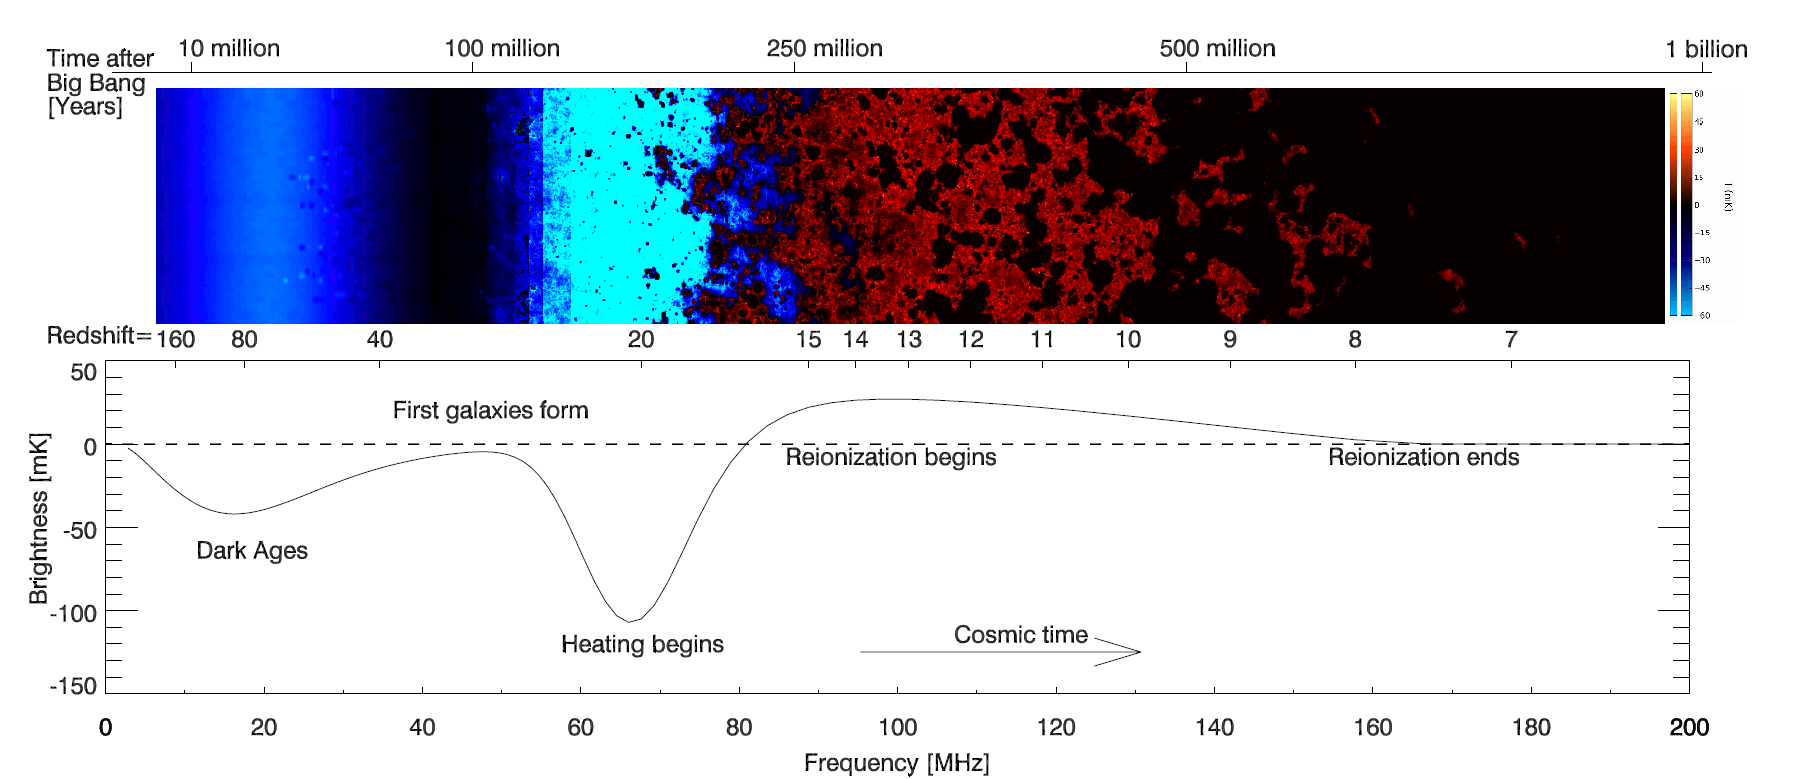
\includegraphics[scale=0.3]{history1.png}
    \caption{}
    \label{historyofHI}
\end{figure}

The mean brightness temperature $T_b$ of the 21cm line can be estimated using 
\begin{equation}
    T_b = 0.3(1+\delta)(\frac{\Omega_{HI}}{10^{-3}})(\frac{\Omega_m+a^3\Omega_\Lambda}{0.29})^{-1/2}(\frac{1+z}{2.5})^{1/2}\ mK
\end{equation}

where $1+\delta = \rho_g/\bar{\rho}_g$ is the normalized neutral gas density and $a=(1+z)^{-1}$ is the scale factor. The stages of each evolutionary process can be discussed in detail according to the redshift interval in which each stage occurs, roughly as follows:
\begin{itemize}
    \item $200<Z<1000$: The residual electron component after the proton-electron recombination can couple the gas and the CMB together. The high-intensity collisional coupling makes the spin temperature $T_{S}$ and the CMB temperature $T_{\gamma}$ equal, when the bright temperature of the 21cm line is 0 and there is no detectable 21cm signal.
    \item $40<z<200$: The gas cools adiabatically as the universe expands and the kinetic temperature follows $T_K\propto (1+z)^2$, leading to a kinetic temperature below the CMB temperature $T_{\gamma}$. The bright temperature $T_b < 0$ and exhibits an absorption signal. 
    \item $z_*<z<40$: As the expansion of the universe continues, the density of the gas decreases, the strength of the collisional coupling decreases, and the radiative coupling brought about by the CMB makes $T_S=T_{\gamma}$, which is no detectable 21cm signal.
    \item $z_\alpha < z < z_*$: At redshift $z_*$, stars and galaxies begin to form as the first sources of radiation and start emitting $Ly_\alpha$ photons and X-rays. The $Ly\alpha$ flux and HI are coupled by the Wouthuysen field effect. The emission of $Ly\alpha$ photons in this period is not sufficient to heat the gas to a temperature above the CMB background. At this time the 21cm line shows a strong absorption spectrum. At the redshift $z_\alpha$, the $Ly\alpha$ coupling saturates.
    \item $z_h < z < z_\alpha$: After the saturation of the $Ly\alpha$ coupling, the inhomogeneity of the $Ly\alpha$ flow eventually does not continue to affect the 21 cm spectrum. Heating becomes the dominant factor. The fluctuations of the gas temperature is the main cause of the fluctuations of bright temperature. When the kinetic temperature of the gas $T_K$ is close to $T_\gamma$, the hot regions will show the characteristics of emitting 21cm lines. When the redshift reaches $z_h$, every part of the gas region will be heated to $T_K=T_\gamma$
    \item $z_T<z<z_h$: The temperature of the gas is heated above the CMB background temperature and the emission structure of 21 cm can be observed. At this point the 21cm bright temperature is not yet saturated. At this point the percentage of the ionized gas starts to rise and reaches the order of percent. When the redshift reaches $z_T$, the bright temperature is heated to saturation.
    \item $z_r<z<z_T$: The continuous heating makes the kinetic temperature of the gas much larger than the CMB background temperature. At this point, the HII component starts to become important and the inhomogeneity of the ionization region starts to affect the distribution of the 21 cm spectral lines.
    \item $z<z_r$: After reionization, the source of the 21 cm line is a small amount of neutral hydrogen clumps.
\end{itemize}
It is important to note that the redshift bounds for these phases are not clear. For example, There is also a great deal of uncertainty in $z_h$ and $z_\alpha$, for X-ray preheating may allow collisional coupling to be important before the $Ly\alpha$ flux becomes significant, and let $z_h>z_\alpha$. Measuring and delineating these limits with high accuracy is also one of the important tasks in the current 21cm global signal detection and intensity mapping.

After reionization, only about 1\% of the baryonic material is contained in the residual HI fraction ($\Omega_{HI}\sim 0.01$). Although the total percentage of HI after reionization is relatively small, the absolute content is still large enough to be observed. And for HI observations at redshifts z = 1 to 3, the Galactic synchrotron emission as the main foreground is several orders of magnitude smaller than the emission from the 21 cm line. This makes 21cm intensity mapping still possible in this redshift interval. Due to the wide distribution of HI, HI can be used as a tracer material for the large-scale structure of the universe.21cm intensity mapping can replace the traditional observation of galaxies to some extent as a means to study the large-scale structure of the universe.

\subsection{Large scale structure mapping at low redshift}
In order to understand the role of dark energy in cosmology, it is necessary to study the second half of the history of the expansion of the universe, i.e., the redshift $z=0~2$. For the observation of the late cosmic expansion history, many projects have chosen to detect baryon acoustic oscillation (BAO). Because the acousic wave was frozen after the recombination, the wavelength of BAO peak, about $100h^{-1}Mpc$, provides a standard ruler. The observation of the angular size of BAO peak wavelength at different redshift would provide a accurate measurement of the history of the expansion of the universe.



\subsection{Observation of reionization and cosmic dawn at high redshift}

\section{Intensity mapping with FAST}

\end{document}